\documentclass[12pt]{report}

\usepackage{commands}


\begin{document}

\large

\begin{center}
 Math 575 Homework 3\\
 Due 05/10/2023\\
 By Marvyn Bailly\\
\end{center}

\normalsize

\hrule

%---------------%
%---Problem 1---%
%---------------%

%--status--$

\begin{problem}
    Consider the 2-D map
    \begin{equation*}
        \left\{\begin{array}{l}
        x_{n+1} = -x_n + x_n y_n \\
        y_{n+1} = - \frac{y_n}{2} - x_n y_n - x_n^2  
        \end{array}\right.
    \end{equation*}
    Compute the center manifold using a polynomial expansion including terms up to order 3.  Then write down the approximate map on this center manifold, and use a graphical method to determine the stability of the origin for this approximate map.  Based on this result and the appropriate center manifold stability theorem, write down the stability of the origin for the original 2-D system.
\end{problem}

\begin{solution}

    \noindent
    Consider the 2-D map
    \begin{equation}\label{1eq}
        \left\{\begin{array}{l}
        x_{n+1} = -x_n + x_n y_n \\
        y_{n+1} = - \frac{y_n}{2} - x_n y_n - x_n^2  
        \end{array}\right..
    \end{equation}
    We wish to compute the center manifold using a polynomial expansion up to third order. We will consider the fixed point at the origin. First we will compute the Jacobian to be
    \[ 
        J(x_n,y_n) = \begin{bmatrix}
            -1 + y_n & x_n\\
            y_n - 2x_n & -1/2 - x_n
        \end{bmatrix}.
    \]
    Evaluating the Jacobian at the fixed point on the origin
    \begin{align*}
        J(0,0) &= \begin{bmatrix}
            -1 & 0 \\ 0 & -1/2
        \end{bmatrix},
    \end{align*} 
    which has eigenvalues $\lambda_1 = -1$ and $\lambda_2 = -\frac{1}{2}$ with corresponding eigenvectors $(1,0)^T$ and $(0,1)^T$ respectively. Since we have map, the eigenpair of $\lambda_1$ corresponds to the center manifold while the eigenpair of $\lambda_2$ corresponds to the stable manifold. Thus the center manifold is orthogonal to $y$ and we expect the center manifold to be described by a polynomial of the form
    \[ 
        h(x_n) = ax_n + bx_n^2 + cx_n^3 + \O(x_n^4).
    \]  
    Then we have that
    \begin{align*}
        y_n &= ax_n + bx_n^2 + cx_n^3 + \O(x^4)
    \end{align*}
    which implies that
    \[ 
        y_{n+1} = ax_{n+1} + bx_{n+1}^2 + cx_{n+1}^3 + \O(x^4),
        \]
        and substituting Equation \ref{1eq} for $(x_{n+1},y_{n+1})$ yields
        \[ 
            -\frac{y_n}{2} - x_ny_n - x_n^2 = a\paren{-x_n + x_ny_n} + b\paren{-x_n + x_ny_n}^2 + c\paren{-x_n + x_ny_n}^3 + \O(x^4).
            \]
            \begin{figure}
                \centering
                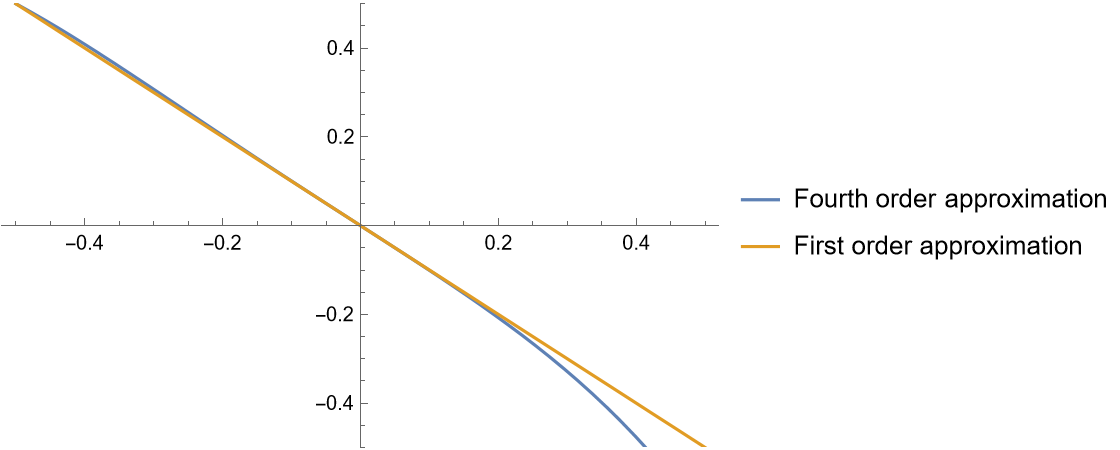
\includegraphics[width=0.75\textwidth,height=\textwidth,keepaspectratio]{images/1.png}
                \caption{Plot of the fourth and first order approximations of the center manifold showing an unstable fixed point at the origin.}
                \label{fig1}
            \end{figure}
    Now substituting $y_n = ax_n + bx_n^2 + cx_n^3 +\O(x^4)$ gives
    \begin{align*}
        -\frac{ax_n + bx_n^2 + cx_n^3}{2} - x_n\paren{ax_n + bx_n^2 + cx_n^3} - x_n^2 &= a\paren{-x_n + x_n\paren{ax_n + bx_n^2 + cx_n^3}}\\ 
        &\quad +b\paren{-x_n + x_n\paren{ax_n + bx_n^2 + cx_n^3}}^2\\ 
        &\quad +c\paren{-x_n + x_n\paren{ax_n + bx_n^2 + cx_n^3}}^3 + \O(x^4)\\
        -\frac{ax_n + bx_n^2 + cx_n^3}{2} - ax_n^2 +bx_n^3 - x_n^2 &= -ax_n + a^2x_n^2 + abx_n^3 + bx_n^2 - 2abx_n^3 - cx_n^3.
    \end{align*}
    Now setting the coefficients of the like terms on the LHS and RHS we see that
    \[ 
        -\frac{a}{2} = -a \implies a = 0,
    \]
    and 
    \[ 
        -\frac{b}{2} - a - 1 = a^2 + b + 2ba \implies b = \frac{-2}{3},    
    \]
    and 
    \[ 
        -\frac{c}{2} + b = ab - c \implies c = -\frac{4}{3}.
    \]
    Plugging $a, b, \and c$ back into the approximation of the center manifold yields
    \[ 
        y = -\frac{2}{3}x^2 - \frac{4}{3}x^3 + \O(x^4).
    \]
    Then plugging $y_n = h(x_n)$ into the Equation \ref{figQ2} gives the approximate map to be 
    \begin{equation*}
            x_{n+1} = -x_n -\frac{2}{3}x_n^3 - \frac{4}{3}x_n^4 + \O(x_n^5).
    \end{equation*}
    Plotting the approximate map along side the first order approximation, as seen in Figure \ref{fig1}, we see that the behavior around the origin is unstable since the slope of the first order approximation is $-1$. Thus starting trajectories around the origin will not converge to the origin. Then by Theorem 18.1.3 we know that the dynamics at the fixed point on the origin is also unstable. 


\end{solution}

%----------------------------------------------------------------------------------------------------%
%\vskip 20pt
\newpage


%---------------%
%---Problem 2---%
%---------------%

%--status--$

\begin{problem}
    Read Chapter 6 of our text (Wiggins) on Index Theory.  Then return to Figure 4.1.2 of the text, and state which of the possible scenarios shown there can be ruled out by index theory, and (very briefly) why.
\end{problem}

\begin{solution}
    
    \begin{figure}
        \centering
        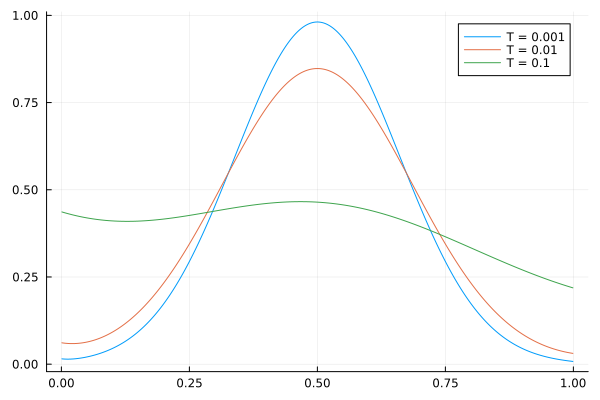
\includegraphics[width=0.75\textwidth,height=\textwidth,keepaspectratio]{images/2.png}
        \caption{Figure 4.1.2 from Wiggins}
        \label{figQ2}
    \end{figure}

    \noindent
    Consider Figure \ref{figQ2} which show a collect of closed orbits that contain fixed points. Since the closed orbit contains at least a fixed point, it is a periodic orbit. Thus Figure \ref{figQ2}b, \ref{figQ2}e, and \ref{figQ2}f can not occur since the index of a periodic orbit must be +1 but each of the closed orbits have an index of 0 since they contain a hyperbolic saddle point which has an index of -1 and a sink/source which has an index of +1 and the index of a closed curve is equal to the sum of the indices. On the other hand, Figure \ref{figQ2}a and \ref{figQ2}d contain one sink/source and thus the index of the periodic orbit is one. For a similar reason, Figure \ref{figQ2}c can also exist since the sum of the index of the fixed points is 1. 

\end{solution}

%----------------------------------------------------------------------------------------------------%
%\vskip 20pt
\newpage

%---------------%
%---Problem 3---%
%---------------%

%--status--$

\begin{problem}
    Read chapter 15 of our text on Gradient Dynamical Systems.  Then, do exercise 15.1.1  Answer this question for flows on $\mathbb{R}^N$. 
\end{problem}

\begin{solution}

    \noindent
    Consider the gradient vector field for $\R^N$ defined by 
    \[
        \dot{x} = - \nabla V(x), \quad x \in \R^N,
    \]
    where the minus sign is picked for traditional purpose can be flipped.
    \begin{enumerate}
        \item [(a)]
        If there is a periodic orbit, then all the points along the orbit are in the $\omega$-limit set of some trajectory $\bar{x}$. Then Theorem 15.0.3., every limit point is a $x$ is an equilibrium point and thus there can not exist a periodic orbit.

        \item [(b)]
        If there is a homoclinic orbit, then the fixed point $\bar{x}$ occurs at the extrema of $V(x)$. If the fixed point occurs at a maxima of $V(x)$, we will consider $\dot{x} = \nabla V(x)$ which places the fixed point at the minima. Then by Theorem 15.0.2, $\bar{x}$ is asymptotically stable, since there exists a neighborhood around $\bar{x}$ that does not contain any other fixed point, namely consider the homoclinic orbit, and thus there can not be a homoclinic orbit since $\bar{x}$ is stable.   
        
        \item [(c)]
        If there is a heteroclinic orbit, then we are considering an orbit between two fixed points, $\bar{x} \and \bar{y}$. We have two cases: either one fixed point is a maxima and the other is a minima, or both fixed points are maxima or minima. In the first case, let $\bar{x}$ be the fixed point that is a minima, then this fixed point is asymptotically stable and will not be able to return to $\bar{y}$. Thus there can not be a heteroclinic orbit in this case. In the other case, if both fixed points are maxima, consider $\dot{x} = \nabla V(x)$ which makes both the fixed point minima. When both the fixed points are minima, then they are both asymptotically stable and once again we can't have heteroclinic orbit with stable fixed points. 
    \end{enumerate}
\end{solution}

%----------------------------------------------------------------------------------------------------%
%\vskip 20pt
\newpage

%---------------%
%---Problem 4---%
%-CUT TUFO POST PRESS. TSZZ DISH. BACK 325 FOR 20-25 
%---------------%

%--status--$

\begin{problem}
    Consider the ``all-to-all'' coupled system of phase oscillators on the N-dimensional torus, with coupling strength $\alpha>0$:
    \begin{equation*}
   \dot \phi_i = - \alpha/N \sum_{j=1}^N f(\phi_j - \phi_i) \mod 2 \pi  
   \end{equation*}
   $i=1...N$.  Show that is a gradient dynamical system when $f(\cdot)$ is an odd function.  Hint:  consider a function $V$ of the form $V = \sum_{i=1}^{N-1} \sum_{j=i+1}^{N} G(\phi_j - \phi_i)$ for an appropriately chosen function $G$. 
\end{problem}

\begin{solution}

    \noindent
    Consider the ``all-to-all'' coupled system of phase oscillators on the N-dimensional torus, with coupling strength $\alpha>0$:
    \begin{equation*}
   \dot \phi_i = - \alpha/N \sum_{j=1}^N f(\phi_j - \phi_i)  
   \end{equation*}
   $i=1...N$ and where $f(\cdot)$ is an odd function. To show that this system is a gradient dynamical system, let's assume $V$ is the function that produces the gradient dynamical system of the form
   \[
        V = \sum_{i=1}^{N-1} \sum_{j=i+1}^{N} G(\phi_j - \phi_i).
   \]
   Then for each $\phi_k$, we have 
   \[
        \pp{V}{\phi_k} = - \sum_{j=1}^{k-1} \pp{G(\phi_k 0 \phi_j)}{\phi_k} - \sum_{j=k+1}^{N}\pp{G(\phi_j - \phi_k)}{\phi_k},
   \]
   and since we are assuming that $V$ defines the gradient dynamical system, $\pp{V}{\phi_k} = \dot{\phi_k}$ which yields
   \begin{align*}
    - \sum_{j=1}^{k-1} \pp{G(\phi_k 0 \phi_j)}{\phi_k} - \sum_{j=k+1}^{N}\pp{G(\phi_j - \phi_k)}{\phi_k} &= - \frac{\alpha}{N}\sum_{j=1}^{k-1}f(\phi_j - \phi_k) - \frac{\alpha}{N} \sum^{N}_{j=k+1}f(\phi_j - \phi_k),
   \end{align*}
   which can be rewritten as
   \begin{align*}
    - \sum_{j=1}^{k-1} \pp{G(\phi_k 0 \phi_j)}{\phi_k} - \sum_{j=k+1}^{N}\pp{G(\phi_j - \phi_k)}{\phi_k} &= \frac{\alpha}{N}\sum_{j=1}^{k-1}f(\phi_k - \phi_j) - \frac{\alpha}{N} \sum^{N}_{j=k+1}f(\phi_j - \phi_k).
   \end{align*}
   Now matching terms, we find that for $j<k$
   \[
        -\pp{G(\phi_k - \phi_j)}{\phi_k} = \frac{\alpha}{N}f(\phi_j - \phi_k),
   \]
   and integrating on both sides and applying the Fundamental Theorem of Calculus yields
   \[
        G(\phi_k - \phi_j) = - \frac{\alpha}{N} \int_{a(\phi_j)}^{\phi_k}f(t - \phi_j)\d t,
   \]
   where $a(\phi_j)$ is some value and $t$ is a dummy variable. Next, we can match terms for $j>k$ which gives
   \[
        \pp{G(\phi_j - \phi_k)}{\phi_k} = \frac{a}{N}f(\phi_j - \phi_k).
   \]
   Combining this result with the $G$ we found prior yields
   \[
    \frac{\alpha}{N}f(\phi_j - \phi_k) = \pp{}{\phi_k}\paren{- \frac{\alpha}{N} \int_{a(\phi_k)}^{\phi_j}f(t - \phi_k)\d t},
   \]
   and using the substitution $u=t + \phi_j - \phi_k$ gives
   \begin{align*}
    \frac{\alpha}{N}f(\phi_j - \phi_k) &= \pp{}{\phi_k}\paren{- \frac{\alpha}{N} \int_{a(\phi_k) + \phi_j - \phi_k}^{2\phi_j - \phi_k}f(u - \phi_u)\d u}\\
    &=\frac{\alpha}{N}f(\phi_j - \phi_k) - \frac{\alpha}{N}(a'(\phi_k) - 1)f(a(\phi_k) - \phi_k).
   \end{align*}
   Then if we let $a(\phi_k) = \phi_k$, we get the desired result for $G$ such that $V$ defines the gradient dynamical system for $\dot{\phi_i}$. Thus we have shown that $\dot{\phi_i}$ is a gradient dynamical system.


\end{solution}

%----------------------------------------------------------------------------------------------------%
%\vskip 20pt
\newpage

%---------------%
%---Problem 5---%
%---------------%

%--status--$

\begin{problem}
    Consider the 2-D flow
    \begin{equation*}
        f = \left\{\begin{array}{l}
        \dot x = y \\
        \dot y = \mu_1 x - x^3 + \mu_2 y - x^2 y  
        \end{array}\right.
    \end{equation*}
    Show that this system has no periodic orbits for any $\mu_1 \in \mathbb{R}$ and $\mu_2 < 0$.
\end{problem}

\begin{solution}
    
    \noindent
    Consider the 2-D flow
    \begin{equation*}
        \left\{\begin{array}{l}
        \dot x = f = y, \\
        \dot y = g = \mu_1 x - x^3 + \mu_2 y - x^2 y.  
        \end{array}\right.
    \end{equation*}
    To rule out periodic orbits for $\mu_1 \in \R$ and $\mu_2 <0$, we will apply Bendixon's theorem, so let's compute $f_x + g_y$ to be
    \[ 
        f_x + g_y = 0 + \mu_2 - x^2.
    \]
    Since $f_x + g_y$ is of the same sign for $\mu_1 \in \R$ and $\mu_2 < 0$, there are no periodic orbits in this region by Bendixon theorem. 


\end{solution}

%----------------------------------------------------------------------------------------------------%
%\vskip 20pt
\newpage

%---------------%
%---Problem 6---%
%---------------%

%--status--$

\begin{problem}
    Wiggins 7.7.7.
\end{problem}

\begin{solution}
    
    \noindent
    Consider the vector field
    \[ 
        \dot{x} = f(x,y,z)
    \]
    where $f(x,y,z)$ is given by the Lorenz equations
    \[
        f(x,y,z) = \begin{cases}
            \dot{x} = \sigma(y - x)\\
            \dot{y} = \rho x - y - xz\\
            \dot{z} = -\beta z + xy,
        \end{cases}
    \]
    for $\sigma, \beta, \rho \geq 0$. Then the divergence of the vector field is
    \[
        \nabla \cdot f = \pp{f_1}{x} + \pp{f_2}{y} + \pp{f_3}{z} = - \sigma - \beta - 1. 
    \] 
    Since $\sigma,\beta > 0$, $\nabla \cdot f \neq 0$ and is everywhere constant. Thus the evolution of volume elements under the flow of this vector field is 
    \[ 
        \dot{V} = cV,
    \]
    where $V(t)$ denotes the volume $D_t = \phi_t(D_0)$ where $D_0$ is some domain within $\R^3$. This has the solution
    \[ 
        V(t) = e^{-(\sigma + \beta + 1)t}V(0),
    \]
    and thus we see that $V(t) \to 0$ as $t \to \infty$, meaning that any initial volume will go to zero as time evolves. 
\end{solution}

%----------------------------------------------------------------------------------------------------%
%\vskip 20pt
\newpage

%---------------%
%---Problem 7---%
%---------------%

%--status--$

\begin{problem}
    Wiggins 7.7.8. Use the definition that a function must be non-constant to count as an integral.
\end{problem}

\begin{solution}
    
    \noindent
    We wish to know if the divergence free property of a vector field implies that the vector field has a fist integral. This is false, consider the following counterexample. Consider the system governed by
    \[ 
        x' = 1,
    \]
    which is divergence free since 
    \[ 
        \nabla \cdot x' = 0.
    \]
    But this system does not have any first integrals. To see why, consider the function $f(x)$ such that 
    \[ \frac{df}{dx} = 1.\]
    Integrating both sides gives 
    \[f(x) = x + C,\] 
    for some constant $C$. However, this function is not constant along the integral curves of $x' = 1$, since the integral curves are simply straight lines with slope $1$. Hence there are no first integrals in this system.
\end{solution}

%----------------------------------------------------------------------------------------------------%
%\vskip 20pt
\newpage

\end{document}